\documentclass[a4paper,12pt]{article}  % Klasa dokumentu
\usepackage[polish]{babel}              % Język dokumentu
\usepackage{amsmath, amssymb}           % Pakiety matematyczne
\usepackage{graphicx}                   % Do wstawiania grafiki
\usepackage{hyperref}                   % Linki w dokumencie
\usepackage{geometry}                   % Ustawienia marginesów
\usepackage{float}
\usepackage[T1]{fontenc}
\usepackage{subfigure}
\usepackage{caption}
\geometry{margin=1in}                   % Definicja marginesów
\usepackage{array}

% Tytuł i autor
\title{Obrazy kanałowe i wskaźniki spektralne}
\author{Adrian Fabisiewicz}
\date{\today}

\begin{document}

\maketitle  % Tworzenie tytułu

\section{Cel zadania}
Celem zadania jest zbadanie:
\begin{itemize}
    \item jak różne klasy obiektów odwzorowują się na obrazach w spektrum widzialnym (RGB) oraz w bliskiej podczerwieni (IR) 
    \item w jaki sposób kompozycje barwne mogą ułatwić interpretację klas obiektów na zdjęciach
    \item roli wskaźników spektralnych w interpretacji obrazów
\end{itemize}

\section{Dane do zadania}
Danymi do zadania były zdjęcia zarejestrowane w zakresie RGB oraz CIR z lat 2015 i 2023 oraz stworzona na ich podstawie poligonowa warstwa wektorowa, zawierająca budynki.

\section{Realizacja}
\subsection{Przedstawienie budynków w poszczególnych kanałach spektralnych}

\subsubsection{Przedstawienie budynku nr 1 w poszczególnych kanałach spektralnych}

\begin{figure}[H]
\hfill
\subfigure[NIR]{
\includegraphics[width=3.5cm]{spektralne/nir_budynek0.png}}
\hfill
\subfigure[RED]{
\includegraphics[width=3.5cm]{spektralne/red_budynek0.png}}
\hfill
\subfigure[GREEN]{
\includegraphics[width=3.5cm]{spektralne/green_budynek0.png}}
\hfill
\subfigure[BLUE]{
\includegraphics[width=3.5cm]{spektralne/blue_budynek0.png}}
\hfill
\end{figure}

\subsubsection{Przedstawienie budynku nr 2 w poszczególnych kanałach spektralnych}

\begin{figure}[H]
\hfill
\subfigure[NIR]{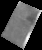
\includegraphics[width=3.5cm]{spektralne/nir_budynek3.png}}
\hfill
\subfigure[RED]{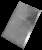
\includegraphics[width=3.5cm]{spektralne/red_budynek3.png}}
\hfill
\subfigure[GREEN]{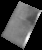
\includegraphics[width=3.5cm]{spektralne/green_budynek3.png}}
\hfill
\subfigure[BLUE]{
\includegraphics[width=3.5cm]{spektralne/blue_budynek3.png}}
\hfill
\end{figure}

\subsubsection{Przedstawienie budynku nr 3 w poszczególnych kanałach spektralnych}

\begin{figure}[H]
\hfill
\subfigure[NIR]{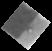
\includegraphics[width=3.5cm]{spektralne/nir_budynek7.png}}
\hfill
\subfigure[RED]{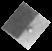
\includegraphics[width=3.5cm]{spektralne/red_budynek7.png}}
\hfill
\subfigure[GREEN]{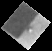
\includegraphics[width=3.5cm]{spektralne/green_budynek7.png}}
\hfill
\subfigure[BLUE]{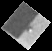
\includegraphics[width=3.5cm]{spektralne/blue_budynek7.png}}
\hfill
\end{figure}

\newpage
\subsection{Zestawienie wybranych statystyk numerycznych w poszczególnych kanałach obrazu.}

\begin{table}[h!]
\centering
\begin{tabular}{|c|c|c|c|}
\hline
\multicolumn{4}{|c|}{\textbf{Obiekt 1}} \\ \hline
\textbf{} & \textbf{min} & \textbf{max} & \textbf{mean} \\ \hline
\textbf{NIR} & 48 & 157 & 77,28289992\\ \hline
\textbf{RED} & 40 & 131 & 70,44365642\\ \hline
\textbf{GREEN} & 43 & 134 & 71,22695035\\ \hline
\textbf{BLUE} & 37 & 120 & 65,39322301\\ \hline
\end{tabular}
\end{table}

\begin{table}[h!]
\centering
\begin{tabular}{|c|c|c|c|}
\hline
\multicolumn{4}{|c|}{\textbf{Obiekt 2}} \\ \hline
\textbf{} & \textbf{min} & \textbf{max} & \textbf{mean} \\ \hline
\textbf{NIR} & 39 & 187 & 101,3616327\\ \hline
\textbf{RED} & 47 & 203 & 127,0130612\\ \hline
\textbf{GREEN} & 60 & 217 & 132,7844898\\ \hline
\textbf{BLUE} & 43 & 205 & 128,0914286\\ \hline
\end{tabular}
\end{table}

\begin{table}[h!]
\centering
\begin{tabular}{|c|c|c|c|}
\hline
\multicolumn{4}{|c|}{\textbf{Obiekt 3}} \\ \hline
\textbf{} & \textbf{min} & \textbf{max} & \textbf{mean} \\ \hline
\textbf{NIR} & 59 & 178 & 90,41953488\\ \hline
\textbf{RED} & 60 & 189 & 98,90325581\\ \hline
\textbf{GREEN} & 55 & 193 & 96,62139535\\ \hline
\textbf{BLUE} & 44 & 191 & 92,05953488\\ \hline
\end{tabular}
\end{table}

\subsection{Porównanie wyglądu obiektów na kompozycjach barwnych RGB, IrGB oraz dwóch innych wybranych kompozycjach.}

\subsubsection{Obiekt 1}
\begin{figure}[H]
\hfill
\subfigure[RGB]{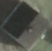
\includegraphics[width=3.5cm]{spektralne/rgb_budynek7.png}}
\hfill
\subfigure[IrGB]{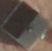
\includegraphics[width=3.5cm]{spektralne/irgb_budynek7.png}}
\hfill
\subfigure[?]{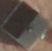
\includegraphics[width=3.5cm]{spektralne/irgb_budynek7.png}}
\hfill
\subfigure[?]{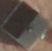
\includegraphics[width=3.5cm]{spektralne/irgb_budynek7.png}}
\hfill
\end{figure}

\subsubsection{Obiekt 2}
\begin{figure}[H]
\hfill
\subfigure[RGB]{
\includegraphics[width=3.5cm]{spektralne/rgb_budynek0.png}}
\hfill
\subfigure[IrGB]{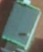
\includegraphics[width=3.5cm]{spektralne/irgb_budynek0.png}}
\hfill
\subfigure[?]{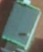
\includegraphics[width=3.5cm]{spektralne/irgb_budynek0.png}}
\hfill
\subfigure[?]{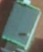
\includegraphics[width=3.5cm]{spektralne/irgb_budynek0.png}}
\hfill
\end{figure}

\subsubsection{Obiekt 3}
\begin{figure}[H]
\hfill
\subfigure[RGB]{
\includegraphics[width=3.5cm]{spektralne/rgb_budynek3.png}}
\hfill
\subfigure[IrGB]{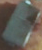
\includegraphics[width=3.5cm]{spektralne/irgb_budynek3.png}}
\hfill
\subfigure[?]{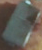
\includegraphics[width=3.5cm]{spektralne/irgb_budynek3.png}}
\hfill
\subfigure[?]{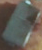
\includegraphics[width=3.5cm]{spektralne/irgb_budynek3.png}}
\hfill
\end{figure}

\subsection{Porównanie wyglądu obiektów na wskaźniku spektralnym NDVI oraz jednym innym wybranym wskaźniku.}
\subsubsection{NDVI}

\begin{figure}[H]
\hfill
\subfigure[Obiekt 1]{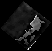
\includegraphics[width=3.5cm]{spektralne/ndvi_budynek7.png}}
\hfill
\subfigure[Obiekt 2]{
\includegraphics[width=3.5cm]{spektralne/ndvi_budynek0.png}}
\hfill
\subfigure[Obiekt 3]{
\includegraphics[width=3.5cm]{spektralne/ndvi_budynek3.png}}
\hfill
\end{figure}

\newpage
\subsection{Zestawienie dla wskaźników spektralnych wartości statystycznych wyznaczonych na danych z 2015 oraz 2023 roku.}

\end{document}
